\documentclass{beamer}
\setbeamercovered{transparent}

\usepackage{epstopdf}
\usepackage[inline]{asymptote}

\mode<presentation> %?

\usetheme{Frankfurt}
\usepackage{helvet}
\usepackage{mathptmx}
%\usefonttheme{professionalfonts}
\usefonttheme[onlymath]{serif}
\usefonttheme{structurebold}

%\renewcommand{\familydefault}{Futura}
%\setsansfont{Verdana}

\setlength{\unitlength}{\paperwidth}

% width, height, title, content
\newcommand{\SizedBlock}[4]{
  \begin{block}{#3}
    \parbox[t][#2\paperwidth][t]{#1\paperwidth}{#4}    
  \end{block}
}

% w1, c1, w2, c2
\newcommand{\TwoColumns}[4]{
  \vspace{-0.02\paperwidth}
  \begin{columns}[t]
    \begin{column}{#1\paperwidth}
      #2
    \end{column}\hspace{-0.02\paperwidth}
    \begin{column}{#3\paperwidth}
      #4
    \end{column}
  \end{columns}
}

% w1, c1, w2, c2, w3, c3
\newcommand{\ThreeColumns}[6]{
  \vspace{-0.02\paperwidth}
  \begin{columns}[t]
    \begin{column}{#1\paperwidth}
      #2
    \end{column}\hspace{-0.07\paperwidth}
    \begin{column}{#3\paperwidth}
      #4
    \end{column}\hspace{-0.07\paperwidth}
	\begin{column}{#5\paperwidth}
      #6
    \end{column}
  \end{columns}
}

% height, title1, content1, title2, content2
\newcommand{\TwoColumnBlocksW}[6]{
  \TwoColumns{
        #6}{
        \SizedBlock{#6}{#1}{#2}{#3}}{
        #6}{
        \SizedBlock{#6}{#1}{#4}{#5}}
}

% height, title1, content1, title2, content2
\newcommand{\TwoColumnBlocks}[5]{
  \TwoColumnBlocksW{#1}{#2}{#3}{#4}{#5}{0.4}
}

% height, title1, content1, title2, content2, title3, content3
\newcommand{\ThreeColumnBlocks}[7]{
  \ThreeColumns{
        0.24}{
        \SizedBlock{0.24}{#1}{#2}{#3}}{
        0.24}{
        \SizedBlock{0.24}{#1}{#4}{#5}}{
        0.24}{
        \SizedBlock{0.24}{#1}{#6}{#7}}
}

\newcommand{\PutPic}[3]{
  \put(#1){\includegraphics[#2\paperwidth]{./img/#3}}
}

\usepackage{color}

\begin{document}
\title{Cost-effective Printing of 3D Objects with Skin-Frame Structures\\
\small{[Weiming Wang.et.al SIG ASIA 2013]}}
\author{Tengfei Jiang}

\newcommand{\FPP}[2]{\frac{\partial #1}{\partial #2}}
\begin{frame}
  \titlepage
\end{frame}

\section{Outline}
\begin{frame}{Outline}
  \begin{enumerate}
    \item Motivation
    \item Background
    \item Key Idea
    \item Algorithm
    \item Results
    \item Concolusion
  \end{enumerate}
\end{frame}


\section{Motivation}
\begin{frame}{Motivation}
\begin{itemize}
\item Material is expensive
\begin{figure}
\centering
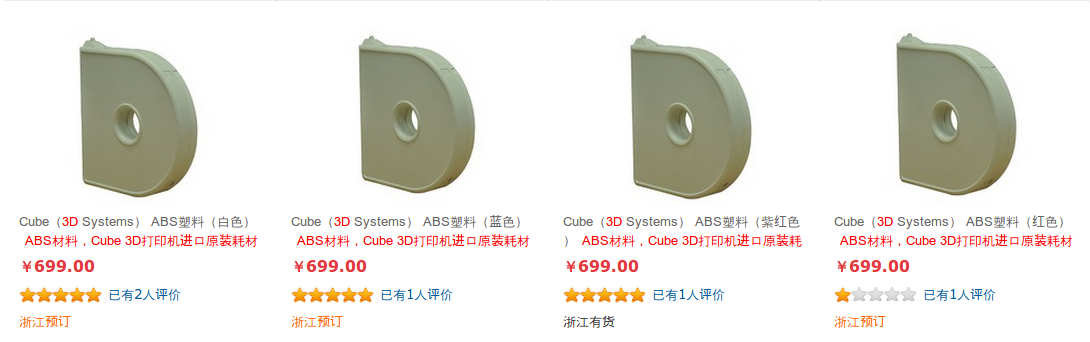
\includegraphics[height=1.2in]{./img/cost.png}
\end{figure}
\end{itemize}
\end{frame}

\begin{frame}{Motivation}
\begin{itemize}
\item Material is expensive
\begin{figure}
\centering
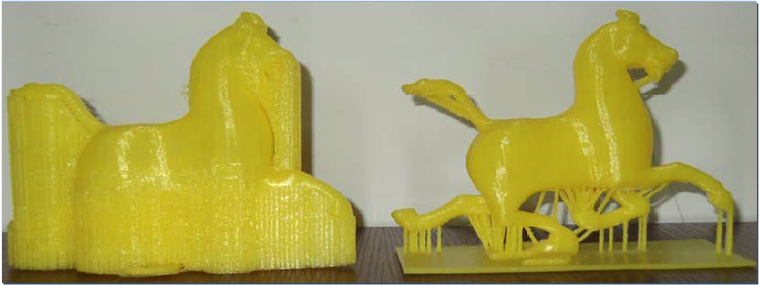
\includegraphics[height=1.2in]{./img/comparison.png}
\end{figure}
\end{itemize}
\end{frame}


\section{Background}
\begin{frame}{Background}
\begin{itemize}
\item Hollowing objects in 3D printing:
\begin{figure}[!htb]
\centering
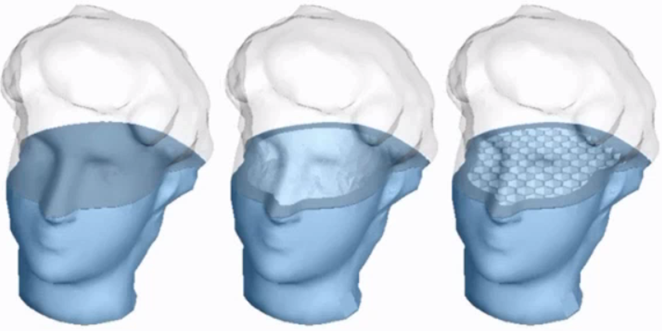
\includegraphics[height=1.0in]{./img/Hollowing.png}
\end{figure}
\item Frame structure:
\begin{figure}[!htb]
\centering
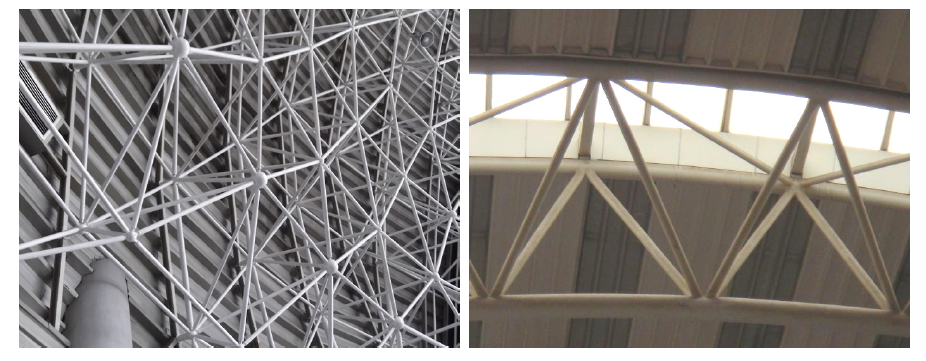
\includegraphics[height=1.0in]{./img/frame-structure.png}
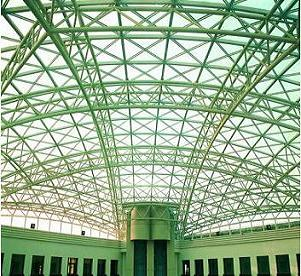
\includegraphics[height=1.0in]{./img/frame-structure-2.png}
\end{figure}
\end{itemize}
\end{frame}

\section{Key Idea}
\begin{frame}{Key Idea}
\begin{block}{Mathematical Modeling}
\begin{figure}[htb]
\centering
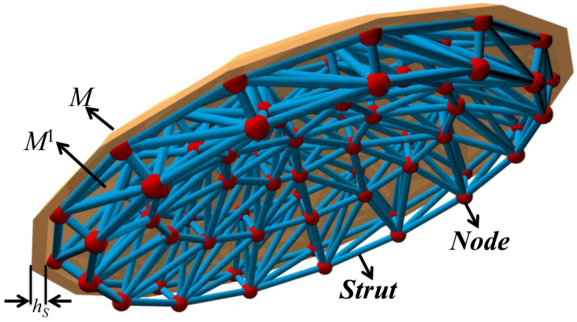
\includegraphics[height=1.2in]{./img/skin-frame.png}
\end{figure}
Goal: minimal Volume and minimal struts.
\end{block}

\begin{block}{Solving}
\begin{itemize}
\item For minimal struts: use $\mathit{L}_0$ optimization.
\item For "goal'' : use multi-objective optimization.
\end{itemize}
\end{block}
\end{frame}

\section{Algorithm}
\begin{frame}{Problem Formulation}
\begin{itemize}
\item Variants: radii $r$ of struts and position $V$ of nodes.
\item Objective: $Vol(r, V, E)$ \& $|E|$
\item Constraints: Printability, Machanics, Geometry\\
Printability: $r\in [\underline{\eta},\bar{\eta}]$
\end{itemize}
\end{frame}

\begin{frame}{Machanics constraints}
\begin{itemize}
\item \textcolor{blue}{Stiffness}: \quad $K(V,r) D = F(r)$ where $K(V,r)$ is stiffness matrix, $D$ is displacement, and $F$ is inner and outer force on each node.
\item \textcolor{blue}{Elastic}: \quad 
\TwoColumns{0.3}{
\begin{figure}[!htb]
\centering
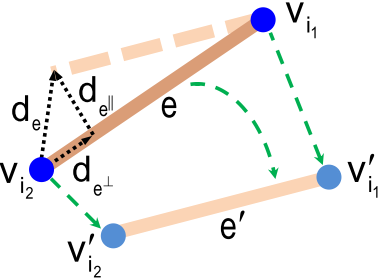
\includegraphics[height=1in]{./img/elastic.png}
\end{figure}
}{0.5}{
\begin{block}{}
\begin{eqnarray}
\|d_{e^{||}}\|/\|e\| \gamma \leq\sigma\\
\|d_{e^{\perp}}\|/\|e\| \mu \leq\tau
\end{eqnarray}
\end{block}
}
\item \textcolor{blue}{Buckling} \quad $r_j\geq l_j/\alpha$, where $\alpha$ is a given slenderness ratio.
\end{itemize}
\end{frame}

\begin{frame}{Geometry constraints}
\begin{itemize}
\item \textcolor{blue}{Geometry Approximation}: $\|d_i\|\leq \epsilon_i$. Deformation of each strut should not larger than a given threshold $\epsilon_i$
\item \textcolor{blue}{Shape Barrier}: $\forall e_i(v_{i_1}v_{i_2})\in E_{int}$
\begin{eqnarray}
v_{i_1},v_{i_2}\in C
\end{eqnarray}
where $C$ is a maximal convex region contains $e_j$ and enclosed by $M^1$. \textcolor{red}{Didn't say how to formulate this constraint.}
\item \textcolor{blue}{Balance}: keep object stand on plane. [Prevost et.al 2013]
\begin{eqnarray}
G_{proj}\in H
\end{eqnarray}
where $G_{proj}$ is the projection of gravity center $G$, and $H$ is a convex hull of its contactpoints on plane.
\end{itemize}
\end{frame}

\begin{frame}{Solving}
Since $\min Vol$ has higher priority than $\min |E|$, straightly formulate them into a single objective optimization will lead to a problem: How to choose an appropriate weight to trade off them?

The problem is splited into two steps:
\begin{itemize}
\item Geometry Optimization:  $\min Vol, \quad s.t.\quad cons$ 
\item Topology Optimization:  $\min |E|, \quad s.t. \quad cons \& Vol\leq \tilde{Vol}$
\end{itemize}
\end{frame}


\begin{frame}{Solving Details}
\begin{figure}[!htb]
\centering
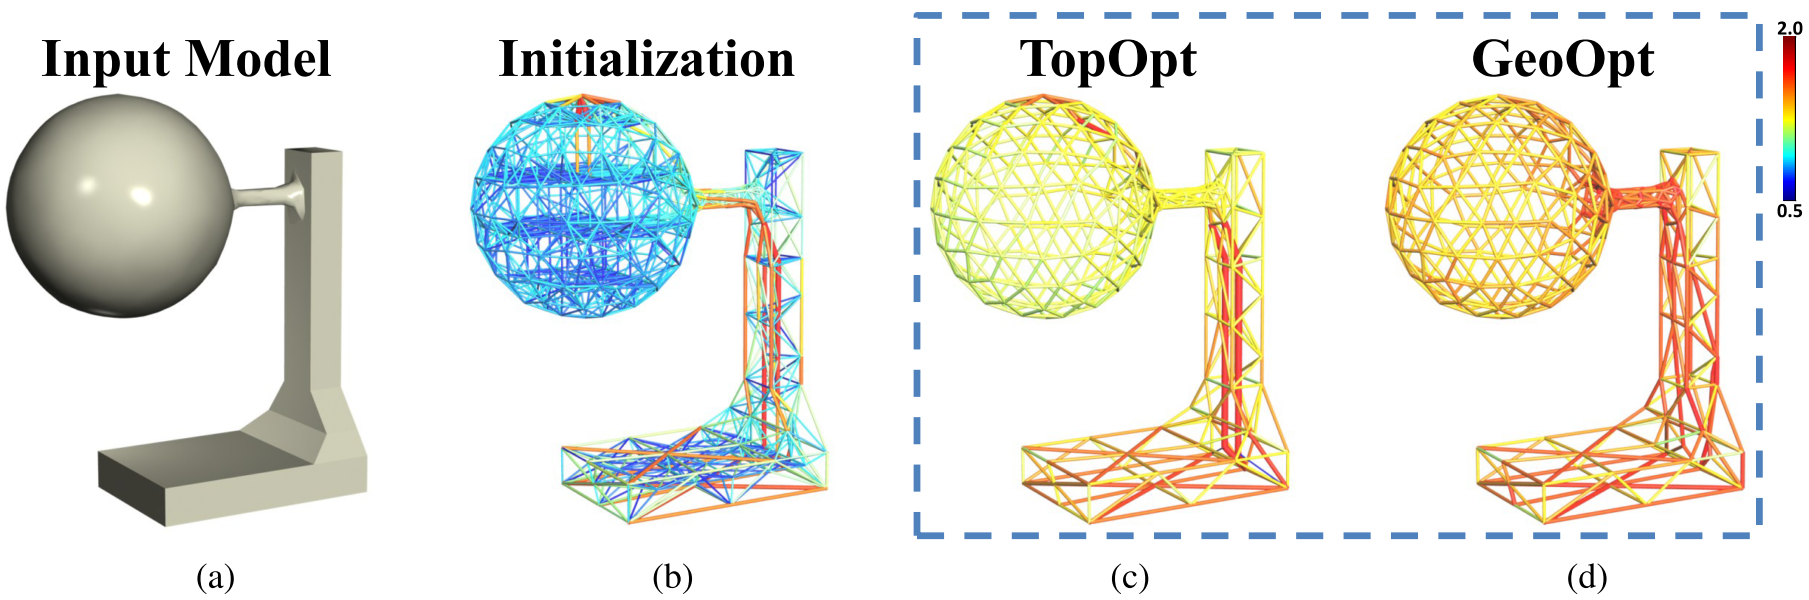
\includegraphics[height=1.5in]{./img/pipeline.png}
\end{figure}
\end{frame}

\begin{frame}{Initialization}
\begin{itemize}
\item Determin node number and position
  \begin{itemize}
    \item Node Number
      \TwoColumns{0.3}{
        \begin{figure}
          \centering
          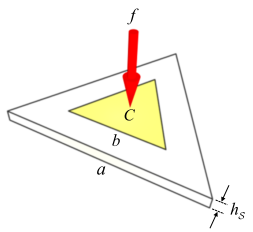
\includegraphics[height=0.8in]{./img/push.png}
        \end{figure}
      }{0.5}{
       \begin{eqnarray}
         d&\approx& f(a-b)/(3\sqrt{3}\mu h_s b)\\
         a&\leq& 3\sqrt{3}\mu h_sb\epsilon/f+b\\
         \to |V_{skin}| &=& 4Area(M^1)/(\sqrt{3}a^2)
       \end{eqnarray}
      }
    \item Adaptive sampling on $M^1$ and even sampling interior.
  \end{itemize}
\item Determin radis of each strut: \\
Size optimization:
\begin{eqnarray}
\min_r Vol(r,V,E)\\
s.t. \quad cons.
\end{eqnarray}
\end{itemize}
\end{frame}

\begin{frame}{Topology Optimization}
\begin{block}{Formulation}
\begin{eqnarray}
\min_r |E_{int}| = \|r_{int}\|_0\\
s.t. \quad cons. \: and\: Vol(r) \leq \tilde{Vol}
\end{eqnarray}

$\|r_{int}\|_0$ is approximated by reweighted $L_1$ minimization:
\begin{eqnarray}
\|Wr\|_1 = W^Tr
\end{eqnarray}
where $r>0$, and $W$ is a diagonal positive definite matrix, $w_i = \frac{1}{\epsilon+(\bar{r}_j-\underline{\eta})}$
\end{block}
\end{frame}

\begin{frame}{Topology Optimization Result}
\begin{figure}
\centering
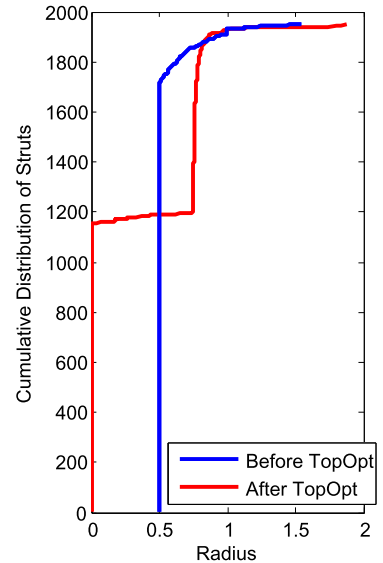
\includegraphics[height=1.7in]{./img/radii.png}
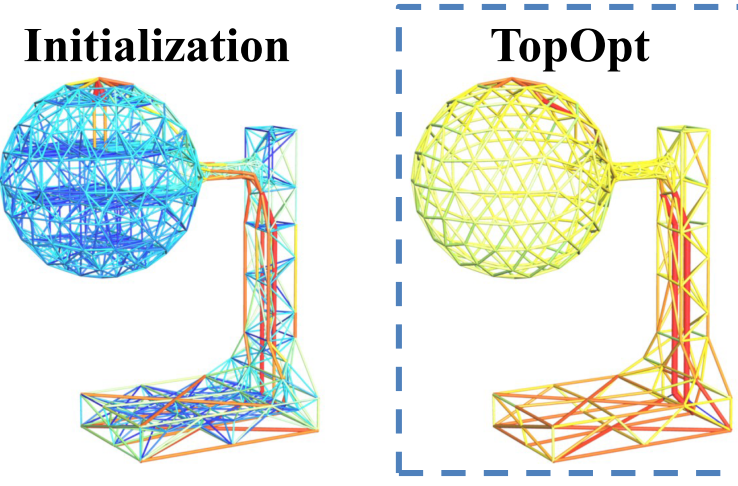
\includegraphics[height=1.7in]{./img/topopt.png}
\end{figure}
Q: Will there be hanging struts?\\
A: No proof.
\end{frame}


\begin{frame}{Geometry Optimization}
\TwoColumns{0.3}{
\begin{figure}
\centering
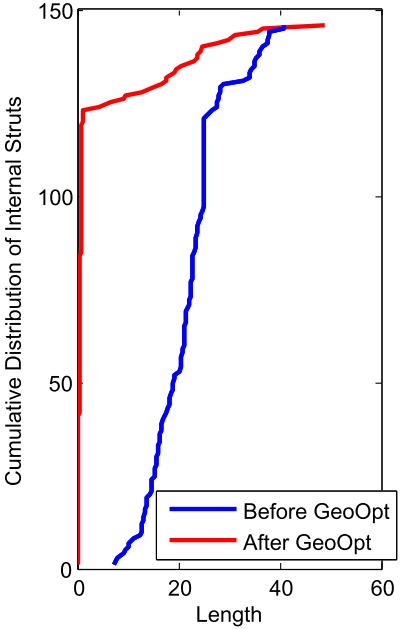
\includegraphics[height=2in]{./img/length.png}
\end{figure}}
{0.5}{
\begin{block}{Formulation}
\begin{eqnarray}
\min_{r,V} Vol(r, V, E)\\
s.t.\quad cons.
\end{eqnarray}
\end{block}
Short length struts will be collapsed.
}
\end{frame}


\begin{frame}{Self supporting}
For extrusion-type 3D printers, extra struts are added for self-supporting.
\TwoColumns{0.2}{
\begin{figure}[htb]
\centering
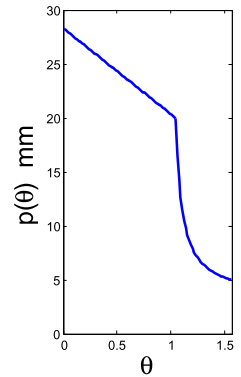
\includegraphics[height=2in]{./img/param.png}
\end{figure}
}{0.6}{
\begin{figure}[htb]
\centering
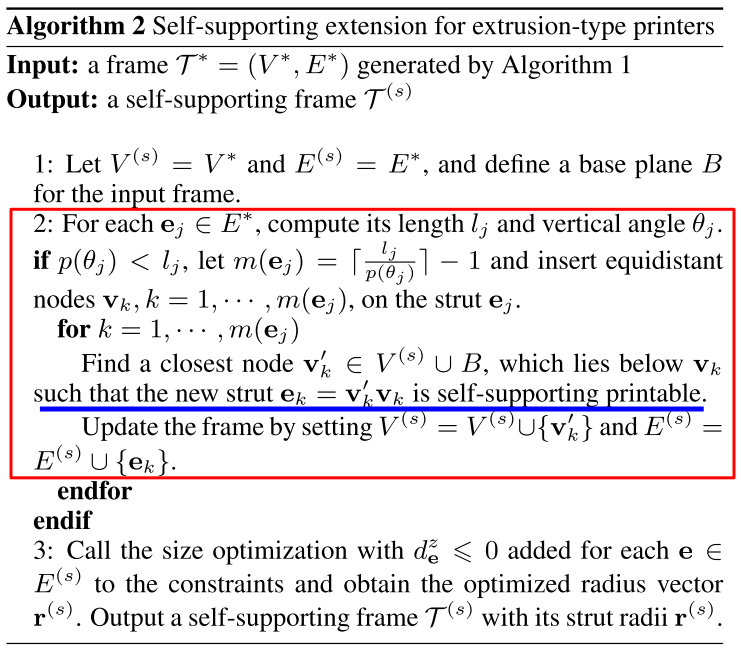
\includegraphics[height=2in]{./img/alg2.png}
\end{figure}
}
\end{frame}

\section{Results}
\begin{frame}{Results}
\begin{figure}
\centering
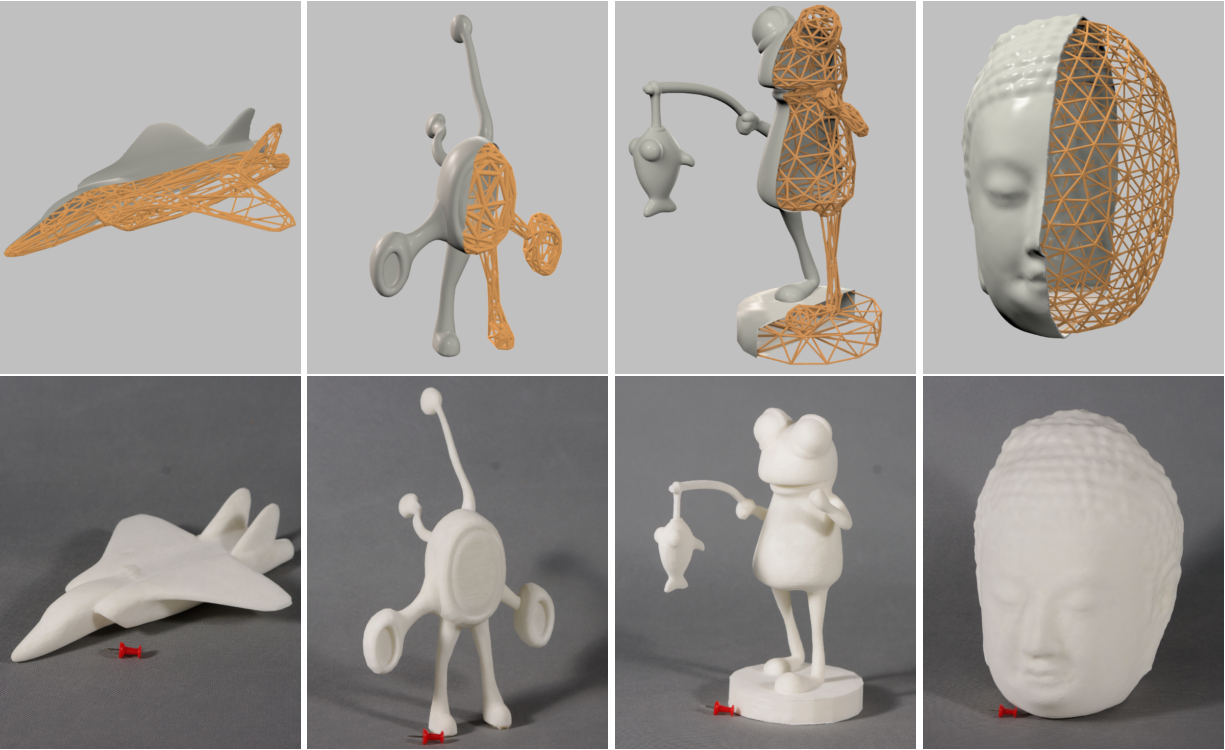
\includegraphics[height=2.5in]{./img/result1.png}
\end{figure}
\end{frame}

\begin{frame}{Results}
\begin{figure}
\centering
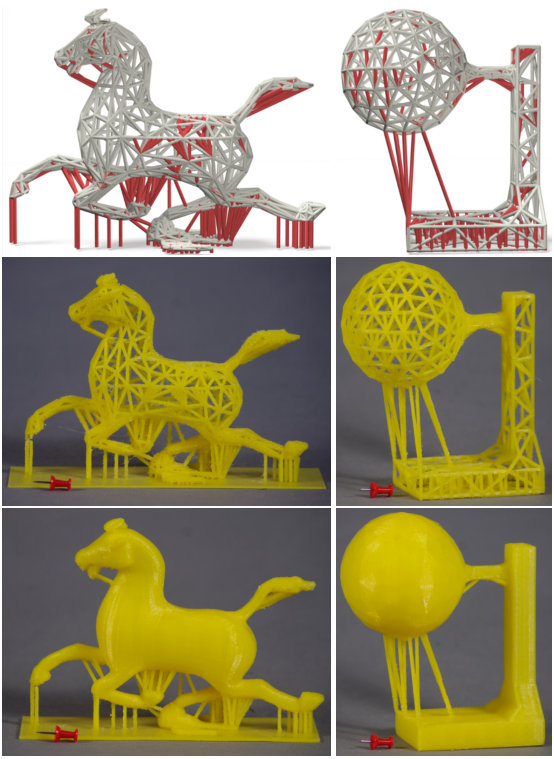
\includegraphics[height=2.8in]{./img/result2.png}
\end{figure}
\end{frame}


\section{Conclusion}
\begin{frame}{Conclusion}
\begin{itemize}
\item First method considering cost-effective printing
\item Nice addressing of approximation of $L_0$ norm.
\item Nice addressing of multi-objective optimization. It's a good try to jump out of local minimal.
\item Future Work:
  \begin{itemize}
    \item Lack of considering orientation.
    \item Only small size could be printed directly, large size model should be segmentated. How to design frame for those models should be considered.
  \end{itemize}
\end{itemize}
\end{frame}

\begin{frame}{}
\hspace{1.5in}\huge{Thank you!}
\end{frame}
\end{document}
